% ---------------------------------------------------------------------------------------------------------------- %
% Architecture
% ---------------------------------------------------------------------------------------------------------------- %
\chapter{Architecture} % (fold)
\label{cha:architecture}

Legacy’s architecture is composed by several entities: the blockchain platform, Legacy’s own infrastructure, an Oracle---which serves as interface between the smart contracts and the outside world---and other third-party services. In an ideal scenario, third-party services would only be required for providing input data to the PoL engine, whereas most of the application logic would reside in the Blockchain. However, given the current state of maturity of blockchain technologies and related services, some functionalities must be initially implemented using a custom backend as well as third-party infrastructure. As a consequence, Legacy’s architecture is expected to evolve in time, starting from a hybrid architecture and converging towards a fully decentralized architecture.
In the long-term, Legacy is expected to operate autonomously---a design goal that is required in order to minimise trust on the Legacy organization and to


\section{Legacy v1.0 (Memoirs): A Hybrid Architecture} % (fold)
\label{sec:legacy_v1_0_memoirs_a_hybrid_architecture}
Legacy v1.0, named \textit{Memoirs}, will be the first stable release of the Legacy Project. This initial version enables secure distribution of memories in the form of digital data, such as pictures, videos, text documents, etc. Since blockchain technologies supporting privacy requirements are still evolving, Legacy Memoirs is based on a hybrid architecture, taking advantage of smart contracts but keeping user data outside of the Blockchain.
A high-level representation of Legacy Memoirs’ architecture is given in Figure \ref{fig:leg_v1_arch}. Legacy’s own infrastructure and frontends are shown in blue, third-party services in green and the blockchain in red. 

There are two main frontends: a web and a mobile application. These are the main interfaces between the user and the core infrastructure, and provide simmilar functionalities so that the service can be fully accessed and configured from either of both.
The web and mobile applications are also employed by the system to obtain PoL data based on user interactions with the service (see also Section~\ref{sub:proof_of_life}).

Legacy’s backend plays different roles. First, it creates smart-contract instances after a user initiates the service and commits a capsule. Second, once a user smart contract is uploaded to the blockchain, the backend sets-up an Oracle instances of running periodic calls in order to execute the code. And third, it also gathers PoL data from external web services and plugins. The user smart contract implements the PoL algorithm that determines if a user is still alive or not, schedules subsequent calls from the backend and triggers the distribution of capsules once the PoL engine determines that the user has died. 
Memories and capsules will be initially stored using third-party services. Further details are given in Section \ref{sub:data_storage}.
To allow our smart contracts to query the outside world (for instance, for PoL signalling), an Oracle interface is required. Legacy Memoirs will employ a third-party, Ethereum-compatible Oracle (such us Oraclize\footnote{http://www.oraclize.it/}).

\begin{figure}[h]
  \centering
  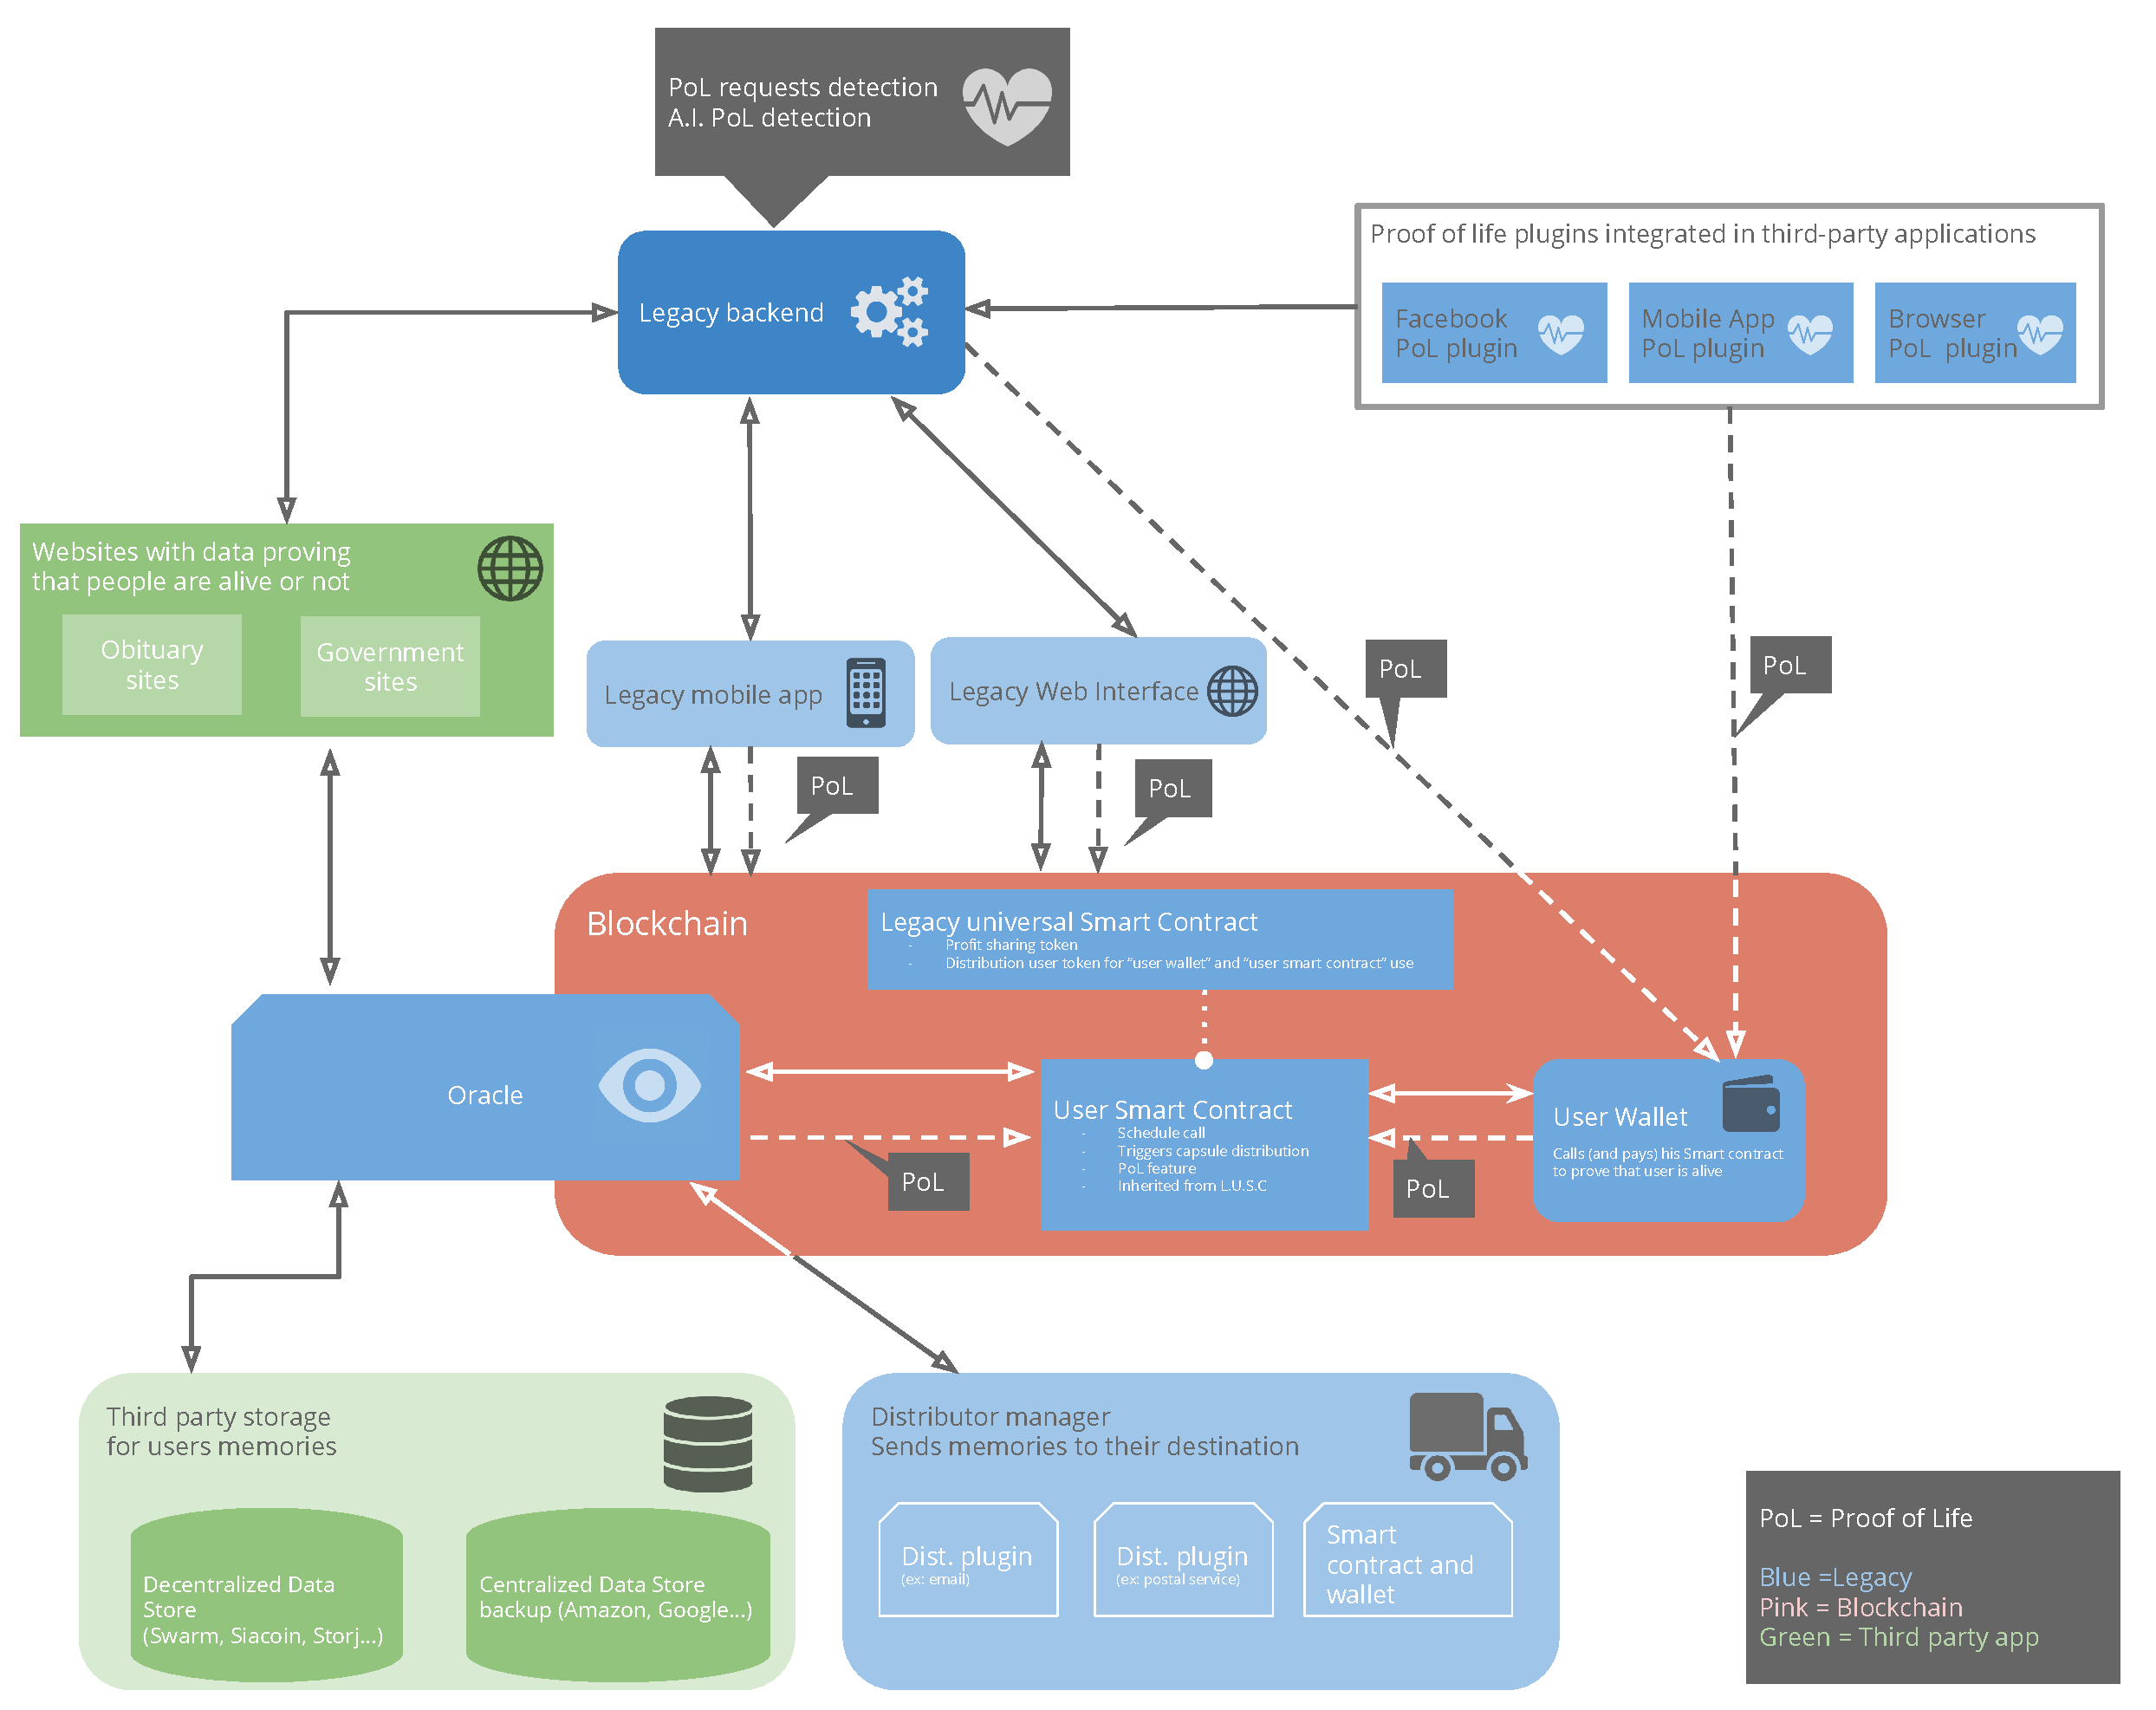
\includegraphics[scale=0.3]{fig/architecture_v02_hybrid}
  \caption{Legacy Memoirs architecture.}
  \label{fig:leg_v1_arch}
\end{figure} 

% subsection legacy_v1_0_memoirs_a_hybrid_architecture (end)

\section{Legacy v2.0 (Heritage): Towards a Fully Decentralized Architecture} % (fold)
\label{sec:legacy_v2_0_heritage_towards_a_fully_decentralized_architecture}
Legacy v2.0 Heritage will be Legacy’s second stable release. Its main differences with respect to Legacy Memoirs are in the underlying architecture. This version intends to take maximum advantage of blockchain features and to minimise dependency on centralized infrastructure.
By this point, we expect to provide support for blockchain-based storage services such as Storj or Siacoin.
In addition, novel blockchain functionalities such as private transactions will be enabled by then and will be likely exploited in Legacy's Heritage. 

% subsection legacy_v2_0_heritage_towards_a_fully_decentralized_architecture (end)

\section{Legacy v3.0 (Future): An Autonomous Platform Based on Rewards} % (fold)
\label{sec:lgacy_v3_0_}

[WIP]
%Allowing the community to develop novel functionalities
% section lgacy_v3_0_ (end)

% \section{Further Releases} % (fold)
% \label{sec:further_releases}
% % TO-DO

% Key aspects that 
% \begin{itemize}
% 	\item Blockchain-agnostic (Cosmos?)
% 	\item Multi-platform and multi-service options (several options for storage, why not)
% \end{itemize}
 


% section further_releases (end)

% chapter architecture (end)